\section{Introduction}

%\begin{figure}[t!]
%\centering
%\includegraphics[width=.9\linewidth]{figures/deploymodel.pdf}
%%\footnotesize
%\vspace{-5pt}
%\caption{The deployment model enabled by \graphenesgx{} to port Linux COTS applications on \sgx{}.
%The framework secures unmodified Linux applications downloaded from official sources, and isolates the applications in enclaves using signatures generated automatically. \fixme{change ``Carbyne'' in this figure}}
%%For each application, \graphenesgx{} can create enclaves without the endorsement of clients,
%%and allows remote servers to verify the execution afterward if necessary.}
%%with the isolation of \sgx{} enclaves.
%%The framework requires no developer's involvement in porting an application to \sgx{}.
%%Instead, it allows centralizing the process of verifying and authenticating applications,
%%to generate signatures needed during enclave creation.
%%In this model, a remote entity who provisions sensitive data
%%can attest the execution of remote enclaves,
%%even if the entity is not the signing authority.
%%\graphenesgx{} is statically linked with {\tt libLinux},
%%the \libos{} binary, and basic libraries of GNU library C.
%%To build up the trust, the \graphenesgx{} image along with
%%a manifest and application measurements
%%are verified by \sgx{} during bootstrap. Applications and other libraries
%%are verified by \graphenesgx{}. The enclave interacts with the host kernel,
%%through untrusted PAL, on a narrowed untrusted interfaces with xx functions.
%%Green (light) boxes and connections represent the components and channels
%%trusted by the owners of sensitive data.
%%Red (dark) ones represent the otherwise.
%%The dotted line indicates that the verification and authentication can be taken offline.
%\label{fig:deploy-model}
%\end{figure}


%The complexity of modern operating systems has become
%a major source of security vulnerabilities,
%pressuring developers to seek solutions to exclude the host OSes
%from their trust models.
%The untrustworthiness of OSes get severe when applications are run in the cloud,
%because the applications may cohabit with compromised tenants,
%or be hosted by malicious providers.


Porting applications to new hardware platforms is difficult.
For instance, \intel{} \sgx{} (Software Guard Extentensions)~\cite{intel-sgx}, 
a new feature on \intel{} CPUs which
%for instance, create an isolated environment, called an {\em enclave},
protects security-sensitive applications against untrusted host systems,
restrict the isolated execution to directly access the system API provided by the host OSes.
To reuse legacy applications without rewriting the logics,
developers need to rely on the existing \sgx{} shielding systems
~\cite{baumann14haven,osdi16scone,shinde17panoply}
to {\em transform} legacy applications to executable packages that can be loaded into enclaves
(i.e., the isolated contexts created by \sgx{}).
A \sgx{} shielding system must interact with the host OS in behalf of the isolated applications,
and shield them from leaking secret information or being infiltrated by the hosts.
Either of the purposes poses tremendous challenges to developing these systems.






%requires the applications to be {\em custom-made} (i.e., {\em made for a specific group of users}) to secure in enclaves.
%At the minimum, a user has to statically compile the applications
%against a system API library, and then sign the binaries using a private key.
%In addition, since a large subset of Linux API cannot be securely supported on these frameworks,
%the intervention of developers is required to customize some applications,
%otherwise porting won't be possible.
%The general support for unmodified legacy applications on \sgx{} still awaits development.
 

The support of system APIs in enclaves are restricted by the \sgx{} hardware limitations, and simultaneously threaten by the attacks potentially launchable from the OSes.
The existing system APIs, such as the Linux system call table and the POSIX API,
are designed under the assumptions that the OSes are trusted and have full control to the application memory.
Neither of the assumptions apply to \sgx{}, since \sgx{} applications are designed to run on untrusted OSes and do not allow the OS to modify or eavesdrop the enclave memory. 
For shielding systems (\scone{}~\cite{osdi16scone} and \panoply{}~\cite{shinde17panoply}) that {\em redirect}
system APIs between the OS and applications,
it is extremely challenging to design defense strategies against
every malicious inputs manipulated by the OSes 
to each API functions.
Although these systems claim that most of the targeted APIs can be supported by redirection, any API functions without reasonable defense against the OSes cannot be considered as usable by applications.



Another type of \sgx{} shielding systems, pioneered by \haven{}~\cite{baumann14haven},
use a {\bf \libos{}} in enclaves to translate the system API from a narrow, easy-to-defend enclave interface.
The enclave interface required by a \libos{} to implement the system API
is smaller in term of both number of entries and complexity of inputs that can be manipulated by the attackers.
Unlike the existing system APIs to export OS states and activities that may leak security-senstive information,
such as file offsets and thread identifiers,
a \libos{} can encapsulate most OS states and activities inside the enclaves,
exporting only the OS states that are known to be defensible, such as file contents (by cryptographical means).



However, despite that shielding systems like \haven{} can thoroughly defend the supported system API, a few challenges to supporting popular system abstractions still remain unaddressed.
For starters, 
multi-process behaviors cannot be natively supported in enclaves due to the restriction on sharing memory.
\haven{} chooses not to address multi-process support because of the type of applications it targets (Windows applications),
but for applications designed on POSIX-compliant OSes, such as Linux and BSD, multi-process abstractions like forking and inter-process communication are actually indispensable~\cite{tsai16apistudy}.
Multi-process support is also a problem to other shielding systems---\scone{} excuses itself from supporting multi-process applications~\cite{osdi16scone}; \panoply{} supports some simple multi-process abstractions including fork, {\tt execve}, signals, and a modified shared-memory abstraction~\cite{shinde17panoply}.
Another problem of \haven{} is delegating the shielding on the enclave interface (e.g., authenticating the loaded binaries) to a trusted, remote server,
because \haven{} cannot trust or verify the inputs from the host OSes.
For desktop users or small business owners, it is uneconomic to maintain a trusted server
just to serve their enclaves.






%In addition, none of the existing \sgx{} frameworks
%provides a library that securely supports a sufficient subset of Linux system APIs for general legacy applications.
%Porting legacy applications with these existing \sgx{} frameworks still requires developers to intervene
%to deal with source code.

%Over the past years, CPU architectures have made significant progress in securing high-value applications
%from the potential risks in the infrastructures.
%A critical milestone is the introduction of isolated execution hardware, including
%TrustZone of ARM~\cite{arm-trustzone},
%SGX (Software Guard Extension) of Intel~\cite{intel-sgx},
%and SecureBlue++ of IBM~\cite{secureblue++}.
%These technologies provide end-to-end protection of applications,
%from establishing the chain of trust with code integrity,
%to complete separation of trustworthy and suspicious execution.
%%Their primary advantage, compared with software solutions,
%%is the defense against unsafe infrastructures under the control of untrusted entities, such as end users or public cloud providers.
%%The hardware-enforced trusted execution is resistant to tampering and bypassing
%%from the host OSes and hardware (except the CPU).
%All these guarantees make isolated execution hardware a promising building block
%for emerging secure systems,
%bringing a surge of interest in utilizing these technologies
%from both research and developer communities.



%%In particular, the design of 
%\intel{} \sgx{} has made exceptional progress in isolating applications from the hosting operating systems.
%%Intel SGX, in particular,
%%is positioned to isolate individual applications with concerns of data confidentiality.
%With \sgx{}, an application can request the creation of an encrypted region in the virtual memory address space---an {\bf enclave} that no one except the CPU can access the execution state.
%%A SGX CPU can trigger
%%an encrypted region---an {\bf ``enclave''}---in the application's virtual memory,
%%to prevent any part of the untrusted host
%%from accessing the data in the region.
%%and ensures all data inside the region to stay encrypted
%%when accessed by untrusted applications or hosts.
%%The key adjustment made by \sgx{} is to exclude operating systems from the ``chain of trust''.
%%and separate each application as the unit of isolation.
%%Essentially SGX excludes the operating systems from the ``chain of trust'',
%%to prevent applications from being compromised by system vulnerabilities, if exploited by co-tenants.
%%Each applications can gain from the isolation tailored to their needs,
%%making \sgx{} a suitable option for data centers.
%%Being tailored to isolating individual applications
%%makes SGX particularly suitable for data centers, as well as other single-user scenarios.
%The exclusion of operating systems from the isolated execution environment 
%brings two primary advantages to applications:
%First, the separation of different applications on a physical machine
%facilitates the usage in data centers for rental and public cloud infrastructure, where multiple tenants share one operating system. 
%%centers, especially a public cloud infrastructure for rental,
%%where different  tenants can share one operating system.
%Besides, a sophisticated, prone-for-mistake monolithic OS can expose applications to unpredictability and vulnerability.
%\sgx{} provides a clean cut of the whole execution environment,
%and resets the system stack that an user has to trust for running sensitive applications.
 

%Despite all the advantages of using \sgx{}, adopting the hardware in modern applications has its caveats.
%%Unfortunately, the advantages of SGX comes with certain caveats.
%%Using the legacy framework (\sdk{}),
%Due to the exclusion of operating systems, all the existing applications that depend on system features and APIs of a legacy operating system will not directly run in an SGX enclave.
%To secure an application that people are familiar with and have paid significant development effort, the users have to ``port'' the application to \sgx{}---customizing the application to address the platform limitations and designing the correspondent isolation strategies.
%%porting an application to an enclave requires
%%developers to adjust the application code fit in the isolation model.
%%The porting effort can be separated into two halves:
%%{\bf the top half} as compartmenting an application for separating sensitive execution from the rest,
%%and {\bf the bottom half} as eliminating the use of OS abstractions and library APIs missing in the infrastructure.
%%The former is based on the expectation of minimizing the trusted computing base, which is often at a best-efforts basis.
%%%and the amount of work for compartmentalization is up to the developers.
%%The bottom half, however, is forced by the restriction of OS interaction in enclaves,
%%which stops most legacy libraries from being reused.
%%%so most legacy libraries that applications used to depend on will be broken inside enclaves.
%%Either kind of the porting effort can cost up to months of development.
%%%especially if the application to isolate contains much privilege separation and OS interaction.
%Using the official framework (the {\bf \sdk{}}),
%porting an application with some level of sophistication is often cumbersome.
%For instance, our experience shows that
%porting a minimal OpenJDK JVM takes roughly three months of a graduate student,
%%For instance, our experience shows that
%%porting a minimal OpenJDK JVM takes roughly three months of a graduate student.
%which is an unacceptable slowdown for an user who asks for immediate adoption of \sgx{}.




%To address the concern,
%isolated execution hardwares such as \sgx{} are introduced
%for the sake of confidentiality and integrity in
%security-sensitive applications,
%upon untrusted hosts.
%\sgx{} supports new instructions to create a
%critical space called {\it enclave} in the application's memory.
%\sgx{} guarantees that only signed code loaded in the enclave can access the critical data,
%and is able to attest the integrity for remote clients.


%How do we make programming for SGX as painless as possible?
%As most developers attempt to adopt SGX in existing applications,
%it is important to allow reuse of most legacy code for the isolated execution.
%Code to reuse includes not only the application itself,
%but all the supporting libraries such as the libc,
%language runtimes (e.g., libstdc++),
%and special-purpose libraries (e.g., OpenSSL).
%Bringing up all these binaries in enclaves requires an infrastructure with sufficient OS compatibility,
%to support all the requested system APIs (i.e., system calls for UNIX).



%Protecting applications without the requirement of trusting the hosts
%has become valuable in modern computer systems for many reasons.
%The complexity of the existing monolithic operating systems has become a major source of
%vulnerabilities to exploit.
%Once the host operating systems are compromised,
%any security mechanisms enforced in the applications can be easily circumvented.
%If the applications run in the cloud,
%the hosts have to be controlled by the cloud providers,
%which is capable of compromising both host operating systems and hardwares.
%The attacks from the cloud is possible even if
%the operating systems' vulnerabilities are never exploited.


%For accelerating the porting process,
%a practical approach is
%to introduce a {\bf \sgx{} shielding layer},
%to provide the required system calls
%and enforce end-to-end, non-partitioned isolation on applications.
%{\bf \haven{}}~\cite{baumann14haven} first introduced the concept,
%by extending a Windows \libos{} called \drawbridge{} to shield an application in an \sgx{} enclave.
%\haven{} contributes a defense strategy against the so-called {\bf Iago attacks}~\cite{checkoway13iago}---when an isolated environment exports all system APIs to a malicious host operating system,
%the host operating system can manipulate the return values of system APIs to compromise the isolated environment. \haven{} prevents the attack by ``absorbing'' the OS components into the enclaves, and leaving a narrow interface to the host OS and the enclave.
%Another work, {\bf \scone{}}~\cite{osdi16scone}
%designs shielding strategies for each Linux system calls atop a \sgx{}-aware Libc.
%Concerning the defense against Iago attacks,
%\scone{} argues that shielding each system calls is not harder than shielding a narrow host interface of a \libos{},
%if the host interface encapsulates too many abstractions and semantics.



%To address the problem of porting effort,
%we started with deriving the concept of a recent work, {\bf Haven}~\cite{baumann14haven},
%one that suggests a plausible model of reusing and protecting COTS (Commercial off-the-shelf)
%applications in SGX enclaves.
%The underlying mechanism of Haven is based on {\bf Drawbridge},
%a {\bf library OS} capable of supporting unmodified applications in the same process.
%In Haven, the Drawbridge library OS is run inside the enclaves as an initial image,
%and be responsible for loading application binaries
%and providing OS features.
%The involvement of library OS is of the essence in this model:
%as the library OS is isolated in the enclave,
%it provides trustworthy OS features in place of the untrusted host OS.
%%Despite that the library OS still exits the enclaves for IO,
%%it can redirect the IO streams to a trusted server, through secure channels validated using hardware attestation.
%In a nutshell,
%Haven brings back the OS to enclaves,
%but realizes it in a form that fits into the restricted, trusted environment.
%%and has a trusted path for establishing the isolation of applications.
%A later work, SCONE~\cite{osdi16scone}, realizes a similar model to isolate Linux applications in SGX enclave. 



%Unfortunately, leveraging \sgx{} for security
%often requires rewriting the applications to a large extent.
%Because the OSes cannot be trusted,
%enclaves are not allowed to directly access any system interface
%for any OS features
%such as files, networks or scheduling.
%Only a limited subset of system library API can be exported in enclaves;
%for example, the software development kit for \sgx{}
%only supports spin-locking as scheduling tool,
%because other primitives require cooperation from the OS.







%This paper focuses on the {\em last mile} of \sgx{} porting---to isolate unmodified Linux applications including
%especially COTS (commercial, off-the-shelf) applications.

%and improve the seamlessness and flexibility of the procedure of porting the applications to \sgx{}.
%We argue that for securing an application that can depend on ``any'' number of system calls, using a \libos{} with a narrow host interface reveals less attack vectors to the host operating systems than shielding individual system calls (as \scone{}).
%The key factor is that many Linux system calls that \scone{} currently does not shield is much harder to design a shielding strategy than files or network connections. 
%Using a \libos{} can wrap all these system calls inside an enclave,
%by untrusting any unauthenticated host abstractions and emulating using the authenticated ones.

%Former \sgx{} shielding layers, including \haven{} and \scone{}, assume the isolation of each application to be separately addressed,
%using a porting procedure requiring centralized effort.
%One user is responsible of studying the application and its security implications,
%packaging the application code into a static executable image
%and maintaining the correspondent validation and provisioning services if necessary.
%The downside of this model is, whenever there is interest in
%adopting a new application to \sgx{},
%users may likely have to wait on others who have the expertise and familiarity
%to undertake the porting procedure.
%The applications ported to \sgx{}, in the form of static executable images, are often hard to share with other users.
%because they are signed by privately-owned keys and the validation or provisioning services only recognize certain signatures.


%In this paper, we apply the same technique of introducing a library OS in enclaves,
%but refocus on a different purpose than Haven or SCONE.
%Instead of focusing on surrounding the COTS applications with isolation,
%our work aims for reducing the effort of prototyping SGX-based solutions in applications.
%We believe Haven or SCONE is not addressing this exact problem,
%because they enforces out-and-out isolation on applications,
%and leaves little flexibility for developers to determine how enclaves are integrated.
%%In other word, developers are forced to choose between two usage models:
%%the legacy framework (Intel SDK), which allows partial isolation and customizing enclave integration,
%%and Haven, which isolates the whole applications without modification.


%We argue that a library OS should be part of the enclave infrastructure,
%to minimize the effort of porting applications (i.e., the bottom half).
%On the other hand, developers should be given liberty to decide how to compartment and integrate enclaves (i.e., the top half).
%For example, a web server (e.g., Apache) can utilize SGX for session separation,
%by running HTTP responders under isolation.
%A library OS can support the web server binaries inside enclaves,
%while the isolated responders still communicates with the coordinator through system IPC.


Summarizing these problems, 
the current strategies to supporting legacy applications in enclaves
is {\em unfriendly} to unprofessional users,
due to either insufficiency to securely support a large portion of system API,
or dependency on trusted, remote servers to surrogate the OS interaction.
The result of these problems is that none of these \sgx{} shielding systems
can take an unmodified application from the store or an installed disk,
and directly secure it in an enclave.
Each of these frameworks requires certainly level of development effort or customization---SCONE and Panoply requires recompiling the application binaries against the system libraries given by the frameworks;
SCONE requires packaging all application binaries into an encrypted archive,
with the decryption key provisioned from a server.
The effort or cost of adopting these frameworks may be acceptable for cloud environment in a large scale,
but can unrealistic to dispersed users, who may use enclave only occasionally.




In many circumstances, securing unmodified legacy applications---especially application binaries that are ready-made in stores---is necessary or beneficial.
%We argue that there are several occasions where
%waiting for experts to port an application is impractical or inefficient,
%and users can benefit from a framework that
%seamlessly transits applications to \sgx{}:
%\begin{compactenum}
For starters, some commercial applications are close-source and only sold in stores.
Before the developers release the \sgx{}-ready versions of these applications, the users won't be able to secure the applications if the existing frameworks don't accept the ready-made binaries.
It is also straightforward to the users if the applications isolated in the enclaves are up-to-date with the same latest bugfixes and features included by the ones in stores.
To keep an application customized for \sgx{} up-to-date,
the developers have to redo the porting process whenever there are any bugfixes or upgrades,
and spend extra bandwidth to redeploy the signed binaries.
%If an application is custom-made and signed by a user,
%she has to redo the porting whenever there is a bugfix and spend extra bandwidth on (re)deploying the binaries.


%We argue that porting applications to \sgx{} does not have to await the intervention of developers. Instead, users should be able to take an off-the-shelf application and secure it in an enclave as it is.
%A framework that supports off-the-shelf applications will
%%be applicable to custom-made applications as the existing \sgx{} frameworks,
%provide more flexibility for applications to use \sgx{}.
%For instance, users can isolate an application under the emergency of processing
%some security-sensitive information,
%and preserve the measurement of the application to be audited later.


%\item When an application has not yet reach the end of
%its development cycle,
%and users want to keep the SGX-ported applications up-to-date with upstream fixes and features.
%
%\item When the application to secure heavily relies on dynamic linking---e.g., loading binaries with {\tt dlopen()},
%or determining calling targets using linking-time functions.
%Statically packaging and authenticating the binaries
%loses important information about the actual flow of execution in the enclaves. For example, adding the PHP engine module to an Apache web server introduces new threats to the execution.
%Remote provisioning servers should be given options to attest these linking decisions.
%
%\item When users want to create a quick throwaway enclave for isolating random applications---because the data to process are too sensitive to lose---and eventually destroy the enclave without any consequences.
%
%\end{compactenum}


%Figure~\ref{fig:deploy-model} shows the deployment model that this paper envisions.
%In this model, users take COTS applications directly from their original sources (app stores, package repositories, software channels), and secure them with \sgx{} enclaves.
%Instead of relying on developers to make the individual effort
%of porting applications to \sgx{},
%the framework can make the collective effort for allowing the applications simply run inside \sgx{} enclaves.
%%Therefore, we exempt local users and remote provisioning servers
%%from coordinating with or undertaking the transition.
%The created enclaves can then communicate with remote provisioning third-parties,
%who will facus on validating the enclave
%and deciding whether to provision the sensitive data.



%When a user or developer signs an application for \sgx{},
%the action initiates two purposes: (1) endorsing the application to be isolated by \sgx{}, (2) allowing other entities to verify the integrity of execution.
%Although signing is inevitable, we argue that the enforcement of isolation and integrity can be decoupled, to provide more options to developing and deploying \sgx{} applications.
%For instance, a user can isolate an application in an enclave without any endorsement,
%but preserve the measurement of the application for auditing afterward.



%Instead of relying developers or experts of each application
%to undertake the porting,
%maintainers can make the collective effort of transiting applications to \sgx{}.
%By simplifying and standardizing the process of verifying and authenticating application binaries,


\begin{figure}[t!]
\centering
\includegraphics[width=.9\linewidth]{deploymodel.pdf}
%\footnotesize
\vspace{-5pt}
\caption{The deployment model enabled by \graphenesgx{} to port Linux COTS applications on \sgx{}.
The framework secures unmodified Linux applications downloaded from official sources, and isolates the applications in enclaves using signatures generated automatically. \fixme{change ``Carbyne'' in this figure}}
%For each application, \graphenesgx{} can create enclaves without the endorsement of clients,
%and allows remote servers to verify the execution afterward if necessary.}
%with the isolation of \sgx{} enclaves.
%The framework requires no developer's involvement in porting an application to \sgx{}.
%Instead, it allows centralizing the process of verifying and authenticating applications,
%to generate signatures needed during enclave creation.
%In this model, a remote entity who provisions sensitive data
%can attest the execution of remote enclaves,
%even if the entity is not the signing authority.
%\graphenesgx{} is statically linked with {\tt libLinux},
%the \libos{} binary, and basic libraries of GNU library C.
%To build up the trust, the \graphenesgx{} image along with
%a manifest and application measurements
%are verified by \sgx{} during bootstrap. Applications and other libraries
%are verified by \graphenesgx{}. The enclave interacts with the host kernel,
%through untrusted PAL, on a narrowed untrusted interfaces with xx functions.
%Green (light) boxes and connections represent the components and channels
%trusted by the owners of sensitive data.
%Red (dark) ones represent the otherwise.
%The dotted line indicates that the verification and authentication can be taken offline.
\label{fig:deploy-model}
\end{figure}



We present {\bf \graphenesgx{}}, a framework for securing unmodified Linux applications, or more specifically, Linux COTS (commercial, off-the-shelf) applications in enclaves.
Inheriting the spirit of \haven{}, our framework uses
a Linux \libos{} called the \graphene{} \libos{}~\cite{tsai14graphene},
to implement not only the Linux API but also the ABI (application binary interface), 
to support dynamic-linked, unmodified ELF binaries.
What \graphenesgx{} is targeting is a framework with an enclave interface completely shielded from the untrusted OSes,
yet sufficient enough to implement a major portion of the Linux specification.
The strategies we take to shield the enclave interface requires no application modification or maintaining trusted, remote servers,
but only minimal configuration effort that can be easily automated or centralized.
Figure~\ref{fig:deploy-model} shows the model we envisions to facilitate porting Linux COTS applications to enclaves.
Users can take applications directly from the original sources (App stores, package repositories, software channels),
and isolate the applications in enclaves using the application signatures downloaded separately.
% and secure them with \sgx{} enclaves.
%Instead of relying on developers to make the individual effort
%of porting applications to \sgx{},
%the framework can make the collective effort for allowing the applications simply run inside \sgx{} enclaves.
%Therefore, we exempt local users and remote provisioning servers
%from coordinating with or undertaking the transition.
The created enclaves can then communicate with other remote servers,
providing trustworthy attestation to earn the trust to receive provisioning of sensitive resources.
%provisioning third-parties,
%who will facus on validating the enclave
%and deciding whether to provision the sensitive data.




%\graphenesgx{} extends \graphene{} \libos{}~\cite{tsai14graphene}---\graphene{} is a system that supports and isolated unmodified Linux applications
%upon a narrow, platform-independent interface to the host operating systems.
%We port \graphene{} to \sgx{}, as a shielding system similar to the \drawbridge{} \libos{} in \haven{}, but providing sufficient Linux compatibility to run commercial Linux applications.
%The choice of securing Linux applications is also beneficial for the majority of public cloud infrastructures,
%which have overwhelmingly chosen Linux as the client OSes~\cite{cloud-market}.






%Figure~\ref{fig:deploy-model} shows the deployment model that this paper envisions.
%In this model, users take COTS applications directly from their original sources (app stores, package repositories, software channels), and secure them with \sgx{} enclaves.
%Instead of relying on developers to make the individual effort
%of porting applications to \sgx{},
%the framework can make the collective effort for allowing the applications simply run inside \sgx{} enclaves.
%%Therefore, we exempt local users and remote provisioning servers
%%from coordinating with or undertaking the transition.
%The created enclaves can then communicate with remote provisioning third-parties,
%who will facus on validating the enclave
%and deciding whether to provision the sensitive data.


The design of \graphenesgx{} primarily addresses two critical challenges:
% of securing Linux COTS applications with \sgx{}.
First, securing the dynamic loading of unmodified Linux binaries,
while retaining the application integrity to be attestable to remote entities.
Unlike \haven{} relying on the uniqueness of encryption keys to secure application binaries,
\graphenesgx{} generates application signatures that are truly unique to the run-time executables of the applications.
%avoids tying each COTS application
%to a privately-owned signing key that only serves one customer or purpose.
%As a result, enclaves with the identical initial state are distinguishable for remote provisioning entities---\graphenesgx{} overcomes this limitation
%by making the initial enclave state unique to the result of dynamic loading;
%in other word, generating the enclave signatures based on
%which application binaries will be loaded.
Second, \graphenesgx{} narrows and simplifies the enclave interface until we can manually iterate through the interface design and guarantee only inputs that are deterministic and predictable can be passed into the enclaves.
We show that the narrowed enclave interface is sufficient to implement a major portion of the Linux system API,
including unmodified multi-process abstractions such as 
%Another challenge of securing Linux COTS applications is the sufficiency of \libos{} to support system features and APIs.
%Beside just building a \libos{} with complete API support,
%\graphenesgx{} must also shield the system APIs from all potential threats from the untrusted hosts, including Iago-type attacks.
%One type of Linux system APIs that is especially cumbersome to support and secure is the multi-process abstractions---including the creation of multiple process (
forking, {\tt execve}, signaling, pipes, message queues, semaphores, and namespace coordination.
As a requirement for multi-process applications, \graphenesgx{} spans the application processes across multiple enclaves,
to emulate the same separation in native Linux.
Using the multi-process support organically brought by the \graphene{} \libos{}, \graphenesgx{} only has to secure a simple pipe-like RPC abstraction on the host, in order to isolate the complex OS states coordinated among enclaves.

%The Linux multi-process abstractions expose new attack surface to \sgx{} enclaves, if each process has to run inside a separate enclave (obligated for position-dependent executables and applications partitioned into small processes).
%Using the \graphene{} \libos{}, \graphenesgx{} can implement Linux multi-process abstractions, based on a distributed POSIX design coordinated over inter-enclave pipes. \graphenesgx{} effectively shields the multi-process abstractions by authenticating the pipes using \sgx{}'s attestation feature.



%Our platform specifically targets Linux applications.
%Haven is designed to support Windows applications,
%%whereas no similar solution is released for Linux.
%%The lack of porting framework for Linux applications is an enormous missed opportunity,
%while Linux has had a higher market share than Windows in cloud computing.
%A recent report shows that Linux OSes (including Ubuntu, Redhat and CentOS) dominate 88.7\% of the Amazon EC2 images, while Windows only yields 7.9\%~\cite{cloud-market}.
%This reveals that porting Linux applications to SGX is generally more valuable than Windows applications.
%Therefore, we extend {\bf \graphene{}}~\cite{tsai14graphene}, a Linux-compliant \libos{},
%as the backbone of our platform.
%A key feature of using \graphene{} is the support of Linux-style, multi-process abstractions,
%such as copy-on-write fork(), namespace coordination, and system V IPC.
%By porting the multi-process support, our platform even provides options unprecedented in prior \sgx{} \libos{}es,
%such as isolating multi-process applications across multiple enclaves.





%\fixme{This part needs to be rewritten}
%We define an enclave loaded with a fully ported the Graphene \libos{} as a {\bf \graphenesgx{}},
%to represent the basic block of isolation.
%The developers can choose to load an application binary into a \graphenesgx{},
%with a configuration to specify how the enclave interacts with the rest of world.
%For instance, a \graphenesgx{} may have to load a library file,
%or transfer data to another enclave through a network connection or a pipe.
%The configuration will include the information required for self-validation of the \graphenesgx{},
%to ensure the integrity of inputed resources (e.g., file content, network payload).
%In conclusion, the integration of \graphenesgx{}s is based on a simple strategy
%to (ab)use inter-process communication (which becomes ``inter-enclave'' or ``enclave-to-process'') and hardware attestation (for mutual verification).


%We develop and evaluate \graphenesgx{} using off-the-shell Intel CPUs (Skylake I5-6500).
%%In fact, the evaluation based on commercial CPUs was unavailable at the time when Haven was published.
%We expect this paper to reveal
%the realistic performance characteristics of in-enclave \libos{}es.
%Based on our analysis,
%we pinpoint several factors that are critical to the enclave performance,
%and provide insights for \libos{}es or applications to improve their design.
%The key factors we identified include memory usage, and the frequency of enclave exit.
%Take memory usage for instance; we observe that the allocation size determines the start-up time, whereas the working set size affects caching and paging overhead.
%Since developers mostly assume the opposite when designing applications and \libos{}es,
%we suggest fine-tuning the \graphenesgx{} will make significant improvement.


%\graphenesgx{} improves the {\em flexibility} of the porting procedure and the {\em sufficiency} of Linux system call support.
%%it simplifies and standardizes the process of accepting a new application to \sgx{}, lowering the bar for utilizing \sgx{} for securing existing applications.
%Besides being used for securing COTS applications,
%\graphenesgx{} also works as a prototyping framework for developers who design new \sgx{} applications.
%Compared with the alternatives, including \sdk{}a nd \scone{},
%\graphenesgx{} offers an enclave infrastructure with more supported Linux system calls and more integration options with the rest of applications. 


The contributions of this paper is as follows:

\begin{compactitem}

\item A framework called \graphenesgx{} to isolate unmodified, Linux COTS applications in enclaves,
providing sufficient Linux compatibility and complete isolation from the untrusted OS.
%A platform (referred to as ``\graphenesgx{}'' for the rest of paper) as basic blocks of porting application binaries under SGX isolation,
%and reusing most of the legacy code and supporting libraries to minimize the development effort.
%\graphenesgx{} extends the \graphene{} \libos{} to support Linux features upon a narrow interface to untrusted hosts.

\item \graphenesgx{} narrows the enclave interfaces until the security of each enclave entries can be studied and reasoned about.
The primary challenges include enforcing attestable application integrity and isolating multi-process abstractions (e.g., fork, IPC, namespaces).

%\graphenesgx{} shields \shieldsyscallnum{} Linux system calls for applications,
%by authenticating the inputed resource (e.g., files) to the host interface.
%Especially, \graphenesgx{} shields multi-process system calls, including \fork{}, \exec{}, signaling, namespaces, and system V IPC, 
%for applications that span across multiple enclaves.

\item Based on the experience of deploying \graphenesgx{} in systems, we identify several challenges in running COTS applications in enclaves, including performance factors and security issues.

%\graphenesgx{} realizes a deployment model (as shown in Figure~\ref{fig:deploy-model}) that transits Linux COTS applications to \sgx{},
%without the individual effort of porting the applications.
%\graphenesgx{} divides up the three goals of \sgx{}: isolating execution, attesting code integrity and authenticating trusted enclaves---\graphenesgx{} centralizes the effort of bootstrapping the isolation, and assists developers to accomplish the other two goals.
\end{compactitem}




%To alleviate the pain of migrating applications to \sgx{},
%recent works like \haven{}~\cite{baumann14haven} provides a mechanism
%of loading native applications into enclaves,
%alongside a library OS (\libos{) }to facilitate rich OS features.
%These systems are called ``shielding systems''~\cite{xu15controlledchannel},
%which means these systems can secure execution environments
%without trusting the host.

%\haven{} effectively migrates native Windows applications to enclaves,
%providing a shortcut for developers
%to easily boost the security of their products.
%However, there are several limitations in \haven{}, including
%excessive trusted computing base (TCB),
%a restrictive model of adapting applications,
%and missing support for Linux or multi-process applications.






%We present \graphenesgx{}, a \libos{}-based shielding system
%targeting Linux multi-process applications,
%as improvement to the \haven{} model of migrating native application to \sgx{}.
%\graphenesgx{} is derived of \graphene{} \libos{}~\cite{tsai14graphene},
%which supports 139 out of 300 Linux system calls.
%\graphene{} runs numbers of popular applications
%such as Apache web server, OpenJDK virtual machine, or shell scripts,
%all of which relies on multi-process abstractions
%such as {\tt fork}, {\tt execve}, signals or System V IPC.



%By supporting Linux multi-process applications,
%\graphenesgx{} simply applies to a broader range of cloud-based applications
%than \haven{}.
%Survey shows that Linux yields a market share of up to 75 percent in
%enterprise cloud providers~\cite{linuxcloud2014}.
%This data suggests majority of the existing cloud users can
%more easily adopt \graphenesgx{} than \haven{}.




%\graphenesgx{} uses a different model from \haven{}
%to bootstrap the trust of loaded applications.
%\haven{} builds up the trust by packing all binaries
%in an encrypted virtual disk,
%with secret key provisioned consensually from a remote server
%trusted by the clients.
%Contrastingly, \graphenesgx{} relies on a model directly derived from
%the trust model of \sgx{},
%by including applications' checksums
%into the enclave measurement to be attested by hardware.
%\graphenesgx{} can migration applications for enclaves off-line,
%and share binaries (e.g., shared libraries) to save bandwidths for deployment.




%Security-wise speaking,
%\graphenesgx{} provides a way to reduce the TCB of enclaves,
%with a smaller code footprint
%and applications natively partitioned as processes.
%\haven{} in general yields a large TCB
%including a \libos{} as large as 209MB,
%and application binaries around 10s \textasciitilde 100s of MB.
%The image of \graphenesgx{} is merely 10MB,
%and Linux applications generally follow the principle of dividing
%code into smaller, more testable binaries.
%\graphenesgx{} isolates multiple binaries (or processes) of an application
%in separate enclaves, and authenticates inter-process coordination
%by binary-based policies.
%Even if an enclave is compromised, other enclaves of the same application
%can still stay secure as long as
%critical information never flows to the victim.


%\graphenesgx{} provides cloud users
%ease of shielding Linux applications
%and flexibility of implementing any desired security model
%suitable for each binary.


\graphenesgx{} is released as an extension to the open-source \graphene{} project in June 2016~\cite{graphene-github}.
The project is adoption by multiple institutions and corporations, helping people to accelerate \sgx{} development, testing, and research.




